\documentclass[tikz,border=8pt]{standalone}
\usepackage{amsmath}
\usepackage{pgfplots}
\pgfplotsset{compat=1.18}
\definecolor{ink}{HTML}{21352F}
\definecolor{teal}{HTML}{087F7B}
\definecolor{gold}{HTML}{C58B2A}
\definecolor{blue}{HTML}{4B77A8}
\definecolor{rose}{HTML}{B65A62}
\begin{document}
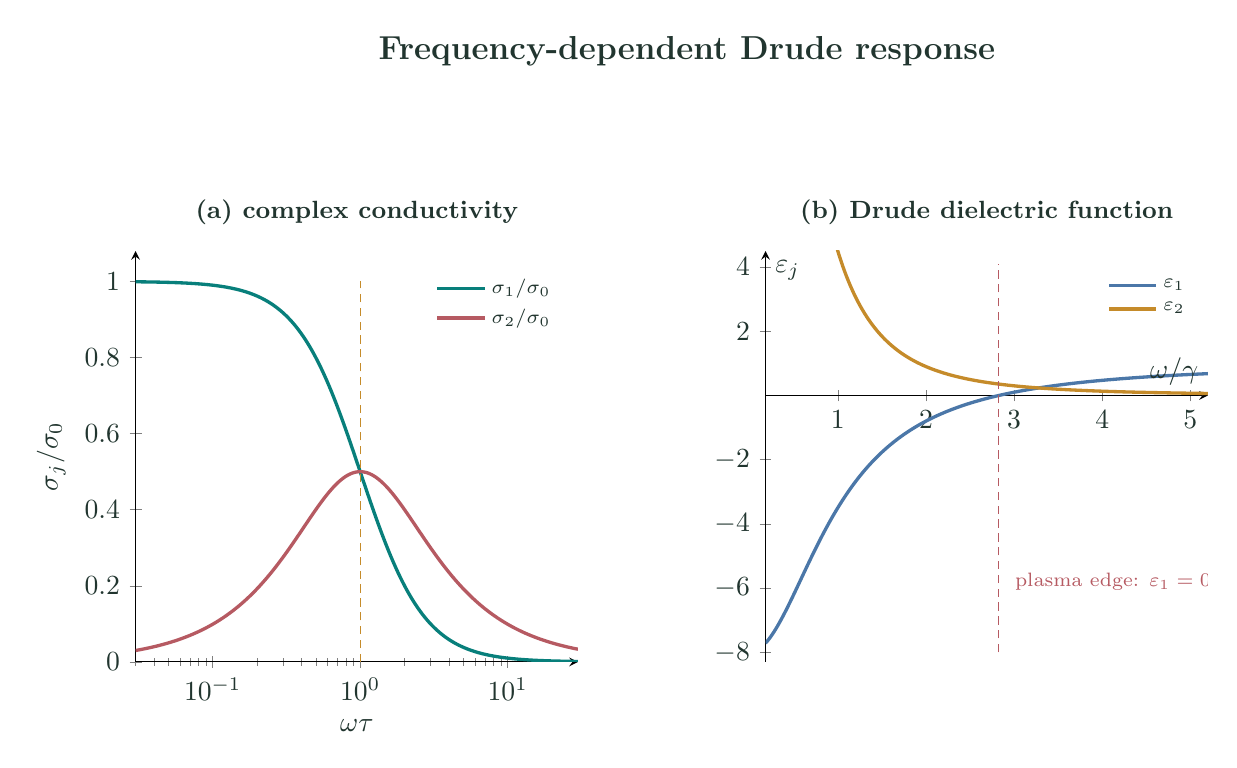
\begin{tikzpicture}[font=\sffamily,text=ink]
  \node[font=\bfseries\large] at (0,4.35) {Frequency-dependent Drude response};
  \begin{axis}[
    at={(-7cm,-3.4cm)},anchor=south west,width=7.2cm,height=6.8cm,
    xmode=log,xmin=.03,xmax=30,ymin=0,ymax=1.08,
    axis lines=left,xlabel={$\omega\tau$},ylabel={$\sigma_j/\sigma_0$},
    title={(a) complex conductivity},title style={font=\bfseries\small},
    legend style={draw=none,fill=none,font=\scriptsize,at={(.97,.96)},anchor=north east}]
    \addplot[teal,very thick,domain=.03:30,samples=220] {1/(1+x^2)};
    \addlegendentry{$\sigma_1/\sigma_0$}
    \addplot[rose,very thick,domain=.03:30,samples=220] {x/(1+x^2)};
    \addlegendentry{$\sigma_2/\sigma_0$}
    \draw[gold,densely dashed] (axis cs:1,0)--(axis cs:1,1.0);
  \end{axis}
  \begin{axis}[
    at={(1cm,-3.4cm)},anchor=south west,width=7.2cm,height=6.8cm,
    xmin=.18,xmax=5.2,ymin=-8.3,ymax=4.5,
    axis lines=middle,xlabel={$\omega/\gamma$},ylabel={$\varepsilon_j$},
    title={(b) Drude dielectric function},title style={font=\bfseries\small},
    legend style={draw=none,fill=none,font=\scriptsize,at={(.98,.96)},anchor=north east}]
    \addplot[blue,very thick,domain=.18:5.2,samples=220] {1-9/(x^2+1)};
    \addlegendentry{$\varepsilon_1$}
    \addplot[gold,very thick,domain=.18:5.2,samples=220] {9/(x*(x^2+1))};
    \addlegendentry{$\varepsilon_2$}
    \draw[rose,densely dashed] (axis cs:2.828,-8)--(axis cs:2.828,4.1);
    \node[rose,font=\scriptsize,anchor=west] at (axis cs:2.9,-5.8) {plasma edge: $\varepsilon_1=0$};
  \end{axis}
\end{tikzpicture}
\end{document}
